\section{La Función Exponencial}
  Para un número complejo $z\in \C$, llamamos {\it representación cartesiana} de $z$ a 
  su expresión como $z = x + iy$, donde $x = \Real(z),\, y =\Imag(z)\in \R$. Recordemos
  también que si $z = x + iy$, entonces su conjugado es $\conj{z} = x - iy$, y se cumple 
  que 
  \[ 
  z \conj{z} = x^2 + y^2 = \abs{z}^2, \,\,\, \abs{z} \text{ es el módulo de } z.
  \]
  Es indispensable también familiarizarnos con la {\it representación polar} $z = re^{i\theta}$.
  Para justificar la expresión de $z$ mediante su módulo y argumento necesitaremos introducir 
  antes la función exponencial compleja.

  \subsection{Definición}
  \begin{defi}
    La función exponencial (que temporalmente denotaremos por $E$) se define por la siguiente serie de
    potencias de radio de convergencia infinito:
    \begin{equation}\label{exp_def}
      E(z) \derDefi \displaystyle \sum_{n=0}^{\infty} \frac{z^n}{n!} \, \cdot
    \end{equation}
  \end{defi}
  El siguiente resultado será de utilidad más adelante, y nos muestra como obtener el producto de Cauchy 
  de dos series con factoriales como denominadores.

  \begin{lemma} \label{lema-cauchy-prod}
    El producto de Cauchy de dos series absolutamente convergentes $\displaystyle\sum_{n=0}^{\infty} \frac{a_n}{n!}$
    y $\displaystyle\sum_{n=0}^{\infty} \frac{b_n}{n!}$ es la serie $\displaystyle\sum_{n=0}^{\infty} \frac{c_n}{n!}$,
    donde los coeficientes $c_n$ están dados por
    \begin{equation}\label{cauchy-prod}
    \displaystyle c_n = \sum_{k=0}^{n} \binom{n}{k}a_kb_{n-k}.
    \end{equation}
    En particular, si las series de potencias $\displaystyle\sum_{n=0}^{\infty} \frac{a_n}{n!}x^n$ y 
    $\displaystyle\sum_{n=0}^{\infty} \frac{b_n}{n!}x^n$ son absolutamente convergentes en $x\in \C$,
    su producto de Cauchy está dado por
    \begin{equation*}
        \displaystyle \left(\sum_{n=0}^{\infty} \frac{a_n}{n!}x^n \right) \left(\sum_{n=0}^{\infty} \frac{b_n}{n!}x^n\right) = 
        \sum_{n=0}^{\infty} \frac{c_n}{n!}x^n,
    \end{equation*}
    donde los $c_n$ son como en \eqref{cauchy-prod}.
  \end{lemma}
  \begin{dem}
    Aplicando la regla para el producto de Cauchy de dos series absolutamente convergentes tenemos que 
    $\displaystyle \frac{c_n}{n!} = \sum_{k=0}^{n} \frac{a_k}{k!}\frac{b_{n-k}}{(n-k)!}$. Por lo tanto,
    \[
    c_n = \sum_{k=0}^{n} \frac{n!}{k!(n-k)!} a_k b_{n-k} = \sum_{k=0}^{n}\binom{n}{k} a_k b_{n-k} \, .
    \]
    La aplicación al caso de series de potencias se sigue de reemplazar $a_n$ y $b_n$ por $a_nx^n$ y $b_nx^n$,
    respectivamente.
  \end{dem}
  Con la ayuda del lema anterior y del teorema del binomio podemos demostrar fácilmente la siguiente ecuación
  funcional de la función exponencial.
  \begin{theo}[Ecuación Funcional] Se verifica la siguiente identidad
    \begin{equation}
        E(z+w) \derDefi E(z)E(w), \quad \forall z,w \in \C.
    \end{equation}
    \begin{dem}
        Haciendo $a_n = z^n$ y $b_n = w^n$ en el Lema \ref{lema-cauchy-prod}, tenemos
        \[
        E(z)E(w) = \sum_{n=0}^{\infty} \frac{c_n}{n!}, \quad \text{con} \quad 
        c_n = \sum_{k=0}^{n} \binom{n}{k}z^k w^{n-k} = (z+w)^n. 
        \]
        Por lo tanto,
        \[
        E(z)E(w) = \sum_{n=0}^{\infty} \frac{1}{n!}(z+w)^n = E(z+w).
        \]
    \end{dem}
  \end{theo}
Como un corolario a la ecuación funcional enunciamos el siguiente teorema, en el cual entre otras cosas
se prueba que $E$ es diferenciable con $E'= E$. 

\begin{theo}\label{teo-propiedades-exp}
    La función exponencial verifica lo siguiente:
    \begin{enumerate}
        \item $E(z)\neq 0$ para todo $z\in \C$.
        \item $\conj{E(z)} = E(\conj{z})$.
        \item $\displaystyle \lim_{h \rightarrow 0} \frac{E(z+h) - E(z)}{h} = E(z)$.
        \item Sean $f: [0,1] \rightarrow \C$ de clase $C^1$, y $F = E(f)$. Entonces, $F$ también es de clase
        $C^1$ en $[0,1]$, con $F' = f'\cdot E(f)$.
    \end{enumerate}
\end{theo}
\begin{dem}
    De la ecuación funcional se sigue que para todo $z\in \C$ se cumple $E(z)E(-z) = E(0) = 1$. Por lo tanto,
    $E(z) \neq 0$, para todo $z\in \C$. La segunda propiedad es consecuencia de que el conjugado se distribuye en 
    sumas y productos, pues
    \[
    \conj{E(z)} = \conj{\sum_{n=0}^{\infty} \frac{z^n}{n!}} = \sum_{n=0}^{\infty}\frac{\conj{z}^n}{n!} = E(\conj{z}).
    \]
    Para la tercera propiedad observemos que cuando $h \rightarrow 0$: 
    \[
    E(z+h)= E(z)E(h) = E(z)\left( 1 + h + \frac{h^2}{2!} + \frac{h^3}{3!} + \cdots \right) = E(z)\left(1+h+ O(h^2) \right),
    \]
    luego, 
    \[
    \frac{E(z+h) - E(z)}{h} = E(z) + O(h) \rightarrow E(z).
    \]
    Por último, si $f\in C^1[0,1]$, entonces 
    \[
    f(t+h) = f(t) + hf'(t) + o(h) \izqDefi f(t) + k.
    \]
    De este modo tenemos
    \[
    F(t+h) - F(t) = E(f(t+h)) - E(f(t)) = E(f(t) + k) - E(f(t)) = E(f(t))\left( E(k) - 1 \right).
    \]
    Luego, 
    \begin{align*}
    F(t+h) - F(t) & =  F(t)(E(k) - 1) = F(t)\left( k + \frac{k^2}{2!} + \cdots \right) = F(t)(k + o(k))\\
                  & = hf'(t)F(t) + o(h),
    \end{align*}
    de donde se sigue el resultado.
\end{dem}

\subsection{La Exponencial Real}
La definición mediante serie de potencias de la exponencial nos permite demostrar el siguiente resultado 
de la exponencial real.

\begin{theo}\label{teo-exponencial-real}
    La función exponencial real $E: \R \rightarrow (0, +\infty)$, es una biyección creciente. En particular, 
    \[
    x<0 \implies E(x) < E(0) = 1, \qquad \text{y} \qquad x>0 \implies E(x) > E(0) = 1. 
    \]
\end{theo}
\begin{dem}
    Por el teorema anterior sabemos que $E: \R \rightarrow \R$ es continua (de hecho diferenciable), y además $E(x)\neq 0$ 
    para todo $x\in \R$, de este modo, por el Teorema de los Valores Intermedios, $E$ es de signo constante (su gráfica nunca cruza el eje $x$). Como
    también sabemos que $E(0) = 1$, entonces $E(x) > 0$ para todo $x\in \R$. Además, para todo $x\in \R$ se cumple 
    $E'(x) = E(x)>0$, por lo tanto $E$ es estrictamente creciente, y por tanto inyectiva. Por último, para mostrar que el rango de $E$ es $(0, \infty)$,
    observemos que $E(x) = 1/E(-x)$, entonces como 
    $\displaystyle\lim_{x \rightarrow \infty} E(x) = \lim_{x\rightarrow \infty} (1+x+\frac{x^2}{2} + \cdots) = \infty$,
    se sigue que $\displaystyle\lim_{x\rightarrow \infty} E(-x) = \lim_{x\rightarrow -\infty} E(x) = 0$. 
\end{dem}

\subsection{La Exponencial Compleja}
El siguiente Lema jugará un rol importante en la prueba del Teorema que le sigue.
\begin{lemma} \label{lema:integral-derivada-logaritmica}
  Sea $\varphi : [0,1]\rightarrow \C^{*} \derDefi \C \setminus \{0\}$, de clase $C^1$, tal que \(\varphi(0) =1\). Y sea 
  \(f: [0,1] \rightarrow \C\) definida por
  \[
  f(x) = \int_{0}^{x} \frac{\varphi'(t)}{\varphi(t)}dt.
  \]
Entonces, \(E(f(x)) = \varphi(x)\) para todo \(x\in [0,1]\) y, en particular, \(\varphi(1)=E(f(1))\).
\end{lemma}
\begin{dem}
  Multiplicando por \(E(-f(x))\) en ambos lados de la igualdad, notamos que \(E(f(x)) = \varphi(x)\) es equivalente a que $1 = \varphi(x)E(-f(x))\izqDefi g(x)$. 
  Basta pues, con demostrar que \(g(x) = 1\) para todo \(x\in [0,1]\).
  Comencemos por observar que \(f(x)\) es de clase $C^1$ (Ejercicio: ¿Por qué?), entonces \(\varphi(x)E(-f(x))\) es diferenciable y
  aplicando el punto 4 del Teorema \ref{teo-propiedades-exp} tenemos que para todo \(x \in [0,1]\):
  \[
  g'(x) = E(-f(x))\left(\varphi'(x) - \varphi(x)\times \frac{\varphi'(x)}{\varphi(x)} \right) = 0.
  \]
  Por tanto, la función \(g(x)\) es constante en \([0,1]\). La demostración termina observando que 
  \(g(0) = \varphi(0)E(-f(0)) = 1\times E(- \int_{0}^{0} \frac{\varphi'(t)}{\varphi(t)}dt) = E(0) =1.\) 
\end{dem}

\begin{theo}\label{teo-propiedades2-exp}
  La función exponencial \(E\) admite las tres propiedades siguientes.
  \begin{enumerate}
    \item Para todo \(z\in \C\) se cumple que \(\abs{E(z)} = E(\Real(z))\).
    \item \(E\) es una función sobreyectiva de \(\C\) sobre \(\C^*\). 
    \item La función \(h: \R \rightarrow \mathbb{T}\vcentcolon = \{\abs{z} = 1\} \), definida por  \(h(t) = E(it) \) es un homomorfismo sobreyectivo. 
    Además se cumple que \( Ker(h) = 2\pi\Z\), donde \(\pi\) es un número positivo.
  \end{enumerate}
\end{theo}
\begin{dem}
   {\bf (1)} Notemos primero que si \(y \in \R \), entonces 
    \[
    \abs{E(iy)}^2 = E(iy)\conj{E(iy)} = E(iy)E(-iy)= E(iy-iy) = E(0) = 1.
    \]
    Entonces, si \(z=x+iy\), se tiene que 
    \[
    \abs{E(z)} = \abs{E(x)E(iy)} = E(x)\abs{E(iy)} = E(x).
    \]
    {\bf (2)} Es en la demostración de este punto que necesitaremos del Lema anterior. 
    Consideremos un \(w \in \C^*\) arbitrario. Vamos a proceder mostrando que existe una
    curva \(\varphi : [0,1] \rightarrow \C^*\) de clase \(C^1\) tal que \(\varphi(0) = 1\)
    y \(\varphi(1) = w\), luego  el Lema nos permite concluir la veracidad del punto {\bf (2)}.
    Es claro que si \(w\) no es un real \(< 0\), entonces el segmento \([1,w]\) no contiene al
    \(0\), y podemos parametrizar este segmento mediante \(\varphi(t) = 1 + t(w-1),\, 0\leq t\leq 1\). Por el Lema anterior
    tenemos que \[w = \varphi(1) = E\left(\int_{0}^{1}\frac{w-1}{1 + t(w-1)}dt\right).\]
    Para el caso en que \(w\) sea un real negativo podemos pensar que basta con tomar \(\varphi(t)\) como una parametrización de un arco
    de circunferencia que una a \(1\) con \(w\), evitando así pasar por el 0. Efectivamente con esto y el Lema anterior se seguiría la prueba. Desafortunadamente 
    todavía no hemos definido lo que son el seno y coseno complejos. Procederemos por otro camino, pero de igual manera terminaremos 
    con un complejo tal que su imagen bajo \(E\) es \(w\).
    Digamos que \(w=-r\) con \(r>0\), comenzamos por observar que \(i \not \in (-\infty, 0)\), 
    luego por lo que recién hemos demostrado existe \(z_0\in \C^*\) tal que \(E(z_0)=i\). 
    Además por el punto (1) se sigue que \(\Real(z_0) = 0\), por lo tanto existe \(\theta_0 \in \R\) tal que \(z_0 = i\theta_0\), 
    es decir, \(i = E(i\theta_0)\).
    Por lo tanto, \(-1 = i^2 = E(2i\theta_0)\), entonces \(w = -r = rE(2i\theta_0)\). Por el Teorema \ref{teo-exponencial-real} tenemos que
    existe \(x\in \R\) tal que \(E(x) = r\), por tanto, \(w = E(2i\theta_0 + x) \). 
    \begin{figure}[H]
        \centering
        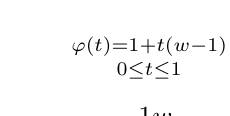
\begin{tikzpicture}[scale=1]
        
          % Usar tus funciones
          \semiPlanoComplejoCentrado{-3}{0}
          %\discoAbierto{1}{1}{1.5}{0.3}
          \punto{-2}{0}{below}{\(1\)}
          \segmentoAzul{-2}{0}{-1}{2}{}
          \punto{-1}{2}{above right}{\(w\)}
          \node at (-0.3,1) {\(\scriptstyle\varphi(t) = 1 + t(w-1)\)};
          \node at (-0.3,0.7) {\(\scriptstyle 0\leq t \leq 1\)};
          %\regionConexa{{(0.5,0) (1,1.2) (1.5,1) (1.8,0.5) (1.7,-1.5) (1,-1) (0.5,-0.3)}}
          \semiPlanoComplejoCentrado{4}{0}{}
          \punto{2}{0}{below}{\(\scriptstyle w = -r \)}
          \punto{5}{0}{below}{\(1\)}
        
        \end{tikzpicture}
        \caption{Para todo \(w\in \C^*\) existe \(z\in \C\) tal que \(E(z)=w\).}
    \end{figure}
    {\bf (3)} Por {\bf(1)} tenemos que \(h\) envía \(\R\) a \(\T\). Recíprocamente, para \(w\in\T\) por {\bf (2)} tenemos que existe
    \(z\in \C\) tal que \(E(z)= w\). Por {\bf (1)} tenemos que \(E(\Real(z)) = \abs{w} = 1\), de donde \(\Real(z) = 0\), y por tanto, \(z= i\theta\)
    para algún \(\theta \in \R\). Con lo que \(h\) es sobreyectiva. Ahora que \(h\) es un homomorfismo se sigue de la ecuación funcional de \(E\).
    Además, \(h\) es continua luego su kernel de \(Ker(h) = \{ t\in \R \tq h(t)=1\}\) es un {\it subgrupo cerrado} de \(\R\). Por lo tanto, 
    \(Ker(h) = \R\) o \(Ker(h) = a\Z\) para algún \(a>0\). El primer caso es imposible, pues hemos visto que existe \(\theta_0 \in R\) tal que
    \(E(i\theta_0) = i\). De aquí se sigue que \(Ker(h) = a\Z\), finalmente definamos \(2\pi = a\).
\end{dem}

\begin{notacion}
    A partir de ahora la función exponencial \(E(z)\) la denotaremos por \(e^z\).
\end{notacion}
    

\begin{obs}
\(\T\) no puede ser homeomorfo a un intervalo \(\mathcal{I}\). En efecto, por compacidad tenemos que \(\mathcal{I}\) tendría que 
ser cerrado, digamos \(\mathcal{I} = [\alpha, \alpha + 2\pi]\), y de ser homeomorfos entonces también lo serían \(\T \setminus \{t\}\) e 
\(\mathcal{I}\setminus \beta\), donde \(\beta\) es un punto interior de \(\mathcal{I}\) y \(t\) es su preimagen bajo el supuesto homeomorfismo. 
Pero ahora tenemos que \(\T \setminus \{t\} \) es conexo pero \(\mathcal{I} \setminus \beta \) no lo es. Esto contradice que \(\T\) y \(\mathcal{I}\) puedan
ser homeomorfos. Dicho esto, el siguiente resultado jugará un papel importante en el estudio del logaritmo.
\end{obs}

\begin{theo}
    Sea \(\alpha \in \R\). La función \(h: t \mapsto e^{it}\) es un homeomorfismo entre el intervalo abierto \((\alpha, \alpha + 2\pi)\) y 
    \(\T \setminus \{e^{i\alpha}\}\).
\end{theo}
\begin{dem}
    S.p.g. podemos suponer que \(\alpha = 0\). Por lo que hemos visto hasta el momento sabemos que \(h\) es continua (Teorema \ref{teo-propiedades-exp}: 3), 
    y biyectiva (Teorema \ref{teo-propiedades2-exp}: 3). Solo falta demostrar que \(h^{-1} : \T\setminus \{1\} \rightarrow (0, 2\pi)\) es continua. 
    Utilizando la caracterización de continuidad por sucesiones, basta con demostrar la siguiente implicación:
    \[
        \left(e^{it_n}\xrightarrow[n\to \infty]{} e^{it}\,\, \text{con } t_n, t \in (0, 2\pi)\right) \implies (t_n \xrightarrow[n\to \infty]{} t).
    \]
    Consideremos pues una sucesión \((t_n)_{n=1}^{\infty}\) y un \(t\in (0,2\pi)\) que satisfacen la hipótesis de la implicación anterior, 
    veamos que también se da la conclusión. En efecto, como \((t_n)_{n=1}^{\infty}\) es acotada, existe un punto de adherencia \(\phi\) de \((t_n)\), 
    luego también existe una subsucesión \((t_{n_k})\) que converge a \(\phi\). De que \(e^{it_n}\xrightarrow[n\to \infty]{} e^{it}\) se sigue que 
    \(e^{it_{n_k}}\xrightarrow[n\to \infty]{} e^{it}\). Por unicidad del límite tenemos que \(\lim_{n \to \infty}e^{it} = e^{i\phi} \). Luego por el 
    punto (3) del Teorema \ref{teo-propiedades2-exp} tenemos que \(t= \phi + 2\pi k\) para algún \(k\in \Z\). 
    \begin{pd}
    \(k=0\).
    \end{pd}
    Como \(t_n, t \in (0, 2 \pi )\) para todo \(n\), se sigue que \(\abs{t_n - \pi}, \abs{t - \pi} < \pi\). De aquí se sigue que \(\abs{\phi - \pi}\leq \pi\). Por lo tanto,
    \[
    \abs{2k\pi} = \abs{t - \phi} \leq \abs{t-\pi} + \abs{\pi - \phi}< 2\pi.
    \]
    Esto implica que \(\phi = t\). Por lo tanto, la sucesión \((t_n)\) posee un único punto de adherencia, luego \((t_n)\) converge, y lo hace a tal punto adherente, es decir,
    a \(t\).
\end{dem}

Estamos ahora en la posición de definir las funciones trigonométricas. 

\begin{defi}
    las funciones {\it seno} y {\it coseno} son definidas en \(\R\) mediante:
    \begin{equation*}        
        \begin{split}
        \cos t =  \Real(e^{it}) = \frac{e^{it} + e^{-it}}{2} &= \sum_{n=0}^{\infty} (-1)^n \frac{t^{2n}}{(2n)!}, \\
        \sin t =  \Imag(e^{it}) = \frac{e^{it} - e^{-it}}{2i} &= \sum_{n=0}^{\infty} (-1)^{n} \frac{t^{2n+1}}{(2n+1)!}        
        \end{split}
    \end{equation*}
\end{defi}
Recordemos que estas funciones son reales, \(2\pi\)-periódicas, admiten un desarrollo en serie de potencias de radio infinito, y que a partir de este desarrollo
se pueden extender al plano complejo:
\[
\cos t = \sum_{n=0}^{\infty} (-1)^n \frac{t^{2n}}{(2n)!} = \frac{e^{it} + e^{-it}}{2}, \qquad \sin t = \sum_{n=0}^{\infty} (-1)^{n} \frac{t^{2n+1}}{(2n+1)!}= \frac{e^{it} - e^{-it}}{2i}.
\]

\subsection{Módulo y Argumento de un Número Complejo}
Las propiedades de la exponencial compleja nos permite probar el siguiente teorema.
\begin{theo}[Módulo y Argumento]
    \begin{enumerate}
        \item Cualquier número complejo \(w\neq 0\) se puede escribir como 
        \[
            w=re^{i\theta}, \quad \text{donde}\quad r>0 \quad \text{y}\quad \theta\in \R.
        \]
        Además, \(r=\abs{w}\) y \(\theta\) está determinado \(\pmod{2\pi}\).
        \item Si  \(w=re^{i\theta} \neq 0\) y si \(n\) es un entero \(\geq 1\), entonces \(w\) posee exactamente \(n\) raíces \(n\)-ésimas \(z_k\), \(z_k^n = w\),
        dadas por 
        \[
            z_k = r^{\frac{1}{n}}e^{i\frac{\theta}{n}}e^{2i\frac{k\pi}{n}}, \quad 0\leq k\leq n-1.
        \]
    \end{enumerate}
\end{theo}
\begin{dem}
    {\bf (1).} Consideremos el complejo \(u = w/r\), con \(r = \abs{w}\). Por el Teorema \ref{teo-propiedades2-exp}, 
    página \pageref{teo-propiedades2-exp}, sabemos que existe \(\theta\) tal que \(e^{i\theta} = u\), de donde se sigue
    que \(w = re^{i\theta}\). Que \(\theta\) está determinado \(\pmod{2\pi}\) se sigue del hecho que el kernel del homomorfismo
    de \(\R\) en \(\T\) dado por \(h: t \mapsto e^{it}\) es \(2\pi\Z\).

    {\bf (2).} Es claro que los \(z_k\) son raíces \(n\)-ésimas de \(w\). También es claro que los \(n\) valores son diferentes, pues si tuviéramos
    \(z_j = z_k\) con \(0\leq j < k \leq n-1\), entonces de \(e^{2i\frac{k\pi}{n}} = e^{2i\frac{j\pi}{n}}\) se seguiría que \((2\frac{k\pi}{n} - 2\frac{j\pi}{n}) \in 2\pi\Z \).
    Lo que a su vez implicaría que \(\frac{k-j}{n} = m\), para algún \(m \in \Z\). Esto es, \(n | k-j\) con \(1\leq k-j \leq n-1\). Lo cual es una
    contradicción (¿Por qué?). Finalmente, para ver que no hay más raíces \(n\)-ésimas fuera de las listadas supongamos que \(z= \rho e^{i\varphi}\)
    es tal que \(z^n = w\). Entonces \(\rho^n = r\), así \( \rho = r^{\frac{1}{n}}\), también \(e^{in\varphi} = e^{i\theta}\), de donde 
    \(n\varphi - \theta = 2\pi l \) para algún \(l\in \Z\). Dividiendo \(l\) entre \(n\) tenemos que \(l = nq + k\), con \(0\leq k \leq n-1 \). 
    Por tanto, \(n\varphi = \theta + 2\pi (nq + k) \), esto es, \(\varphi = \theta/n + 2\pi q + 2\pi k / n\). De todo lo anterior obtenemos que 
    \[
    z = \rho e^{i\varphi} = r^{\frac{1}{n}}e^{i(\theta/n + 2\pi q + 2\pi k / n)} = 
    r^{\frac{1}{n}}e^{i\frac{\theta}{n}}e^{2i\frac{\pi k}{n}}e^{2\pi qi} = r^{\frac{1}{n}}e^{i\frac{\theta}{n}}e^{2i\frac{\pi k}{n}},
    \] 
    con \(0\leq k \leq n-1\). Port lo tanto, \(z = z_k\).
\end{dem}

\subsection{Hacia el Logaritmo Complejo}
Una vez establecida la sobreyectividad de \(E:\C \rightarrow \C^* \), una generalización del Lema \ref{lema:integral-derivada-logaritmica}, página 
\pageref{lema:integral-derivada-logaritmica}, que nos será muy útil es la siguiente.

\begin{theo}[Levantamiento]\label{teo-levantamiento-exp}
    Consideremos una función \(\varphi : [a, b]\rightarrow \C^* \), continua y de clase \(C^1\) a trozos, un complejo \(\mu \in \C \), y la función
    \(f: [a, b] \rightarrow \C \) definida por 
    \[
    \displaystyle f(x) = \int_{a}^{x} \frac{\varphi'(t)}{\varphi(t)} dt + \mu.
    \]
    entonces podemos elegir un \(\mu \) de forma tal que \(E(f(x)) = \varphi(x)\) para todo \(x\in [a,b]\).
\end{theo}
\begin{dem}
    Que \(\varphi\) sea de clase \(C^1\) a trozos significa que existe una partición \(a=t_0 < t_1 < \cdots < t_n = b\) tal que
    \(\varphi\) es de clase \(C^1\) en cada subintervalo \([t_j, t_{j+1}]\), pero con posiblemente \(\varphi'(t_j - 0) \neq \varphi'(t_j + 0)\).

    Eligiendo \(\mu\) de tal manera que \(E(\mu) = \varphi(a)\), lo cual es posible gracias al Teorema \ref{teo-propiedades2-exp}, página \pageref{teo-propiedades2-exp}. 
    Vamos a proceder para cada \(j \in \{0,1,2, \dots , n-1 \}\). Para cada \(x\) en el segmento \([t_j, t_{j+1}]\) tenemos que \(f'(x)= \frac{\varphi'(x)}{\varphi(x)}\).
    Por el Teorema \ref{teo-propiedades-exp}, página \pageref{teo-propiedades-exp}, la función \(g(x) = \varphi(x)E(-f(x))\) satisface que 
    \(g'(x)= \varphi'(x)E(-f(x)) + \varphi(x)(-f'(x)E(-f(x))) = f'(x)\varphi(x)E(-f(x)) - \varphi(x)f'(x)E(-f(x)) = 0 \) para \(x \in [t_j, t_{j+1}]\). De aquí se sigue 
    que la función \(g(x)\) es constante en cada intervalo \([t_j, t_{j+1}]\), y de aquí es constante en todo el intervalo \([a, b]\). Pero 
    \(g(a) = \varphi(a)E(-f(a)) = \varphi(a)E(-\mu) = 1\), de donde podemos deducir que \(g(x) = \varphi(x)E(-f(x)) = 1\). Por último, para concluir basta con multiplicar 
    por \(E(f(x))\)
\end{dem}

\begin{obs}
    El Teorema \ref{teo-levantamiento-exp} afirma que la función \(\varphi\) admite un {\it logaritmo continuo}. 
\end{obs}